\documentclass[aspectratio=43]{beamer}
\usetheme{Simple}

\usepackage[UTF8,fontset=fandol]{ctex}
\usepackage{graphicx}
\usepackage{subfigure}
\usepackage{amsmath}
\usepackage{amsfonts}
\usepackage{amssymb}
\usepackage{booktabs}
\usepackage{array}
\usepackage{xcolor}
\usepackage{xurl}
\usepackage{hyperref}
\usepackage{tikz}
\usetikzlibrary{arrows.meta, positioning, shapes.geometric}
\setbeamertemplate{caption}[numbered]
\setbeamertemplate{bibliography item}[text]

\graphicspath{{Figures/}}

\def\meetingname{Research Presentation}
\title{AegisKV: Fault Tolerance for Multi-Agent LLM Systems}
% \subtitle{System design and related work}
\author[Z Zhao]{Zhan Zhao}
\institute[HKBU]{Hong Kong Baptist University}
\date[2026.07.06]{\meetingname\\July 6, 2026}

\hfuzz=100pt
\hbadness=10000
\vfuzz=100pt
\vbadness=10000
\emergencystretch=\maxdimen

\definecolor{hkblue}{RGB}{24,76,133}
\definecolor{softblue}{RGB}{230,240,250}
\definecolor{softgreen}{RGB}{232,245,236}
\definecolor{softred}{RGB}{252,232,230}
\definecolor{softgray}{RGB}{245,246,248}
\definecolor{softyellow}{RGB}{255,247,220}

\newcommand{\smallcard}[2]{%
  \begin{beamercolorbox}[wd=\textwidth,rounded=true,shadow=false,sep=1.0ex]{block body}
    \textbf{#1}\par
    \vspace{0.25ex}
    \scriptsize #2
  \end{beamercolorbox}
}

\newcommand{\tiercard}[4]{%
  \begin{beamercolorbox}[wd=\textwidth,rounded=true,shadow=false,sep=1.0ex]{block body}
    \textbf{#1}\hfill{\scriptsize #2}\par
    \vspace{0.25ex}
    \scriptsize #3\par
    \vspace{0.25ex}
    {\scriptsize\textit{Risk:} #4}
  \end{beamercolorbox}
}

\begin{document}

\begin{frame}[plain]
  \titlepage
\end{frame}

\begin{frame}{Outline}
  \tableofcontents
\end{frame}

%------------------------------------------------------------
\section{Paper Overview}
%------------------------------------------------------------

\begin{frame}{Paper Overview}
  \small
  \begin{block}{Observations}
    1. Multi Agent scenario -> KV Priority \\
    2. Long Context -> High cost while GPU failure -> Fault tolerance ↑
  \end{block}

  \vspace{0.08cm}
  \begin{block}{AegisKV}
    1. Workflow-aware KV backup layer \\
    2. GPUReplica、HostBackup
  \end{block}

  \vspace{0.08cm}
  \begin{block}{Key Points}
    1. Objective：降低 GPU failure 下的 tail workflow completion time。 \\
    2. Scenario：DP, PP, GPU Failure \\
  \end{block}
\end{frame}

\begin{frame}{Workflow-aware KV Priority}
  \small
  代表性 workflow 同时包含串行 main-agent stage 和 fan-out / fan-in subagent stage (claude code / codex / pi):

  \vspace{0.15cm}
  \[
    O_0 \rightarrow \{S_1,S_2,S_3\} \rightarrow O_0
    \rightarrow \{S_4,S_5,S_6\} \rightarrow O_0 .
  \]

  \vspace{0.10cm}
  \begin{columns}[T,onlytextwidth]
    \begin{column}{0.48\textwidth}
      \begin{block}{High-Priority KV}
        \begin{itemize}
          \item High hit rate
          \item Main agent / Long Subagents
        \end{itemize}
      \end{block}
    \end{column}
    \begin{column}{0.48\textwidth}
      \begin{block}{Low-Priority KV}
        \begin{itemize}
          \item Low hit rate
          \item Short Subagents
        \end{itemize}
      \end{block}
    \end{column}
  \end{columns}

  \vspace{0.12cm}
  \footnotesize
\end{frame}

%------------------------------------------------------------
\section{Motivation}
%------------------------------------------------------------


\begin{frame}{Motivation: Failure Impact Varies}

  \begin{figure}
        \centering
        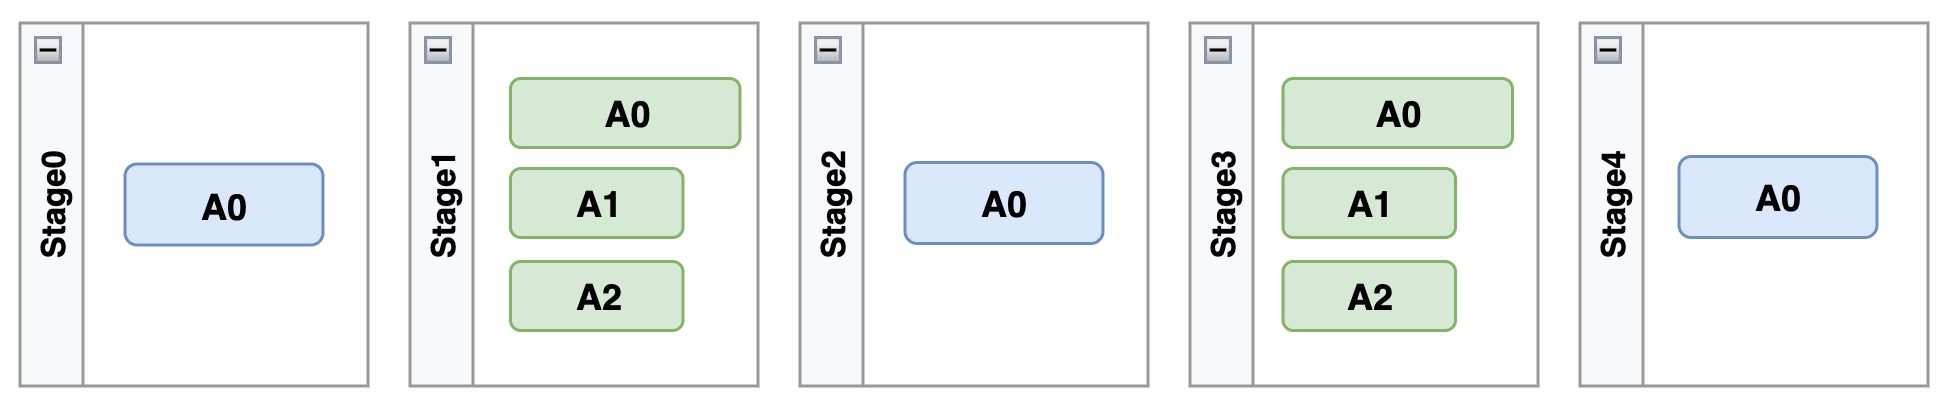
\includegraphics[width=\textwidth]{Figures/agentic_workflow.png}
  \end{figure}
  \vspace{0.4cm}

  \begin{columns}[T,onlytextwidth]
    \begin{column}{0.48\textwidth}
      \vspace{-0.1cm}
      \begin{figure}
        \centering
        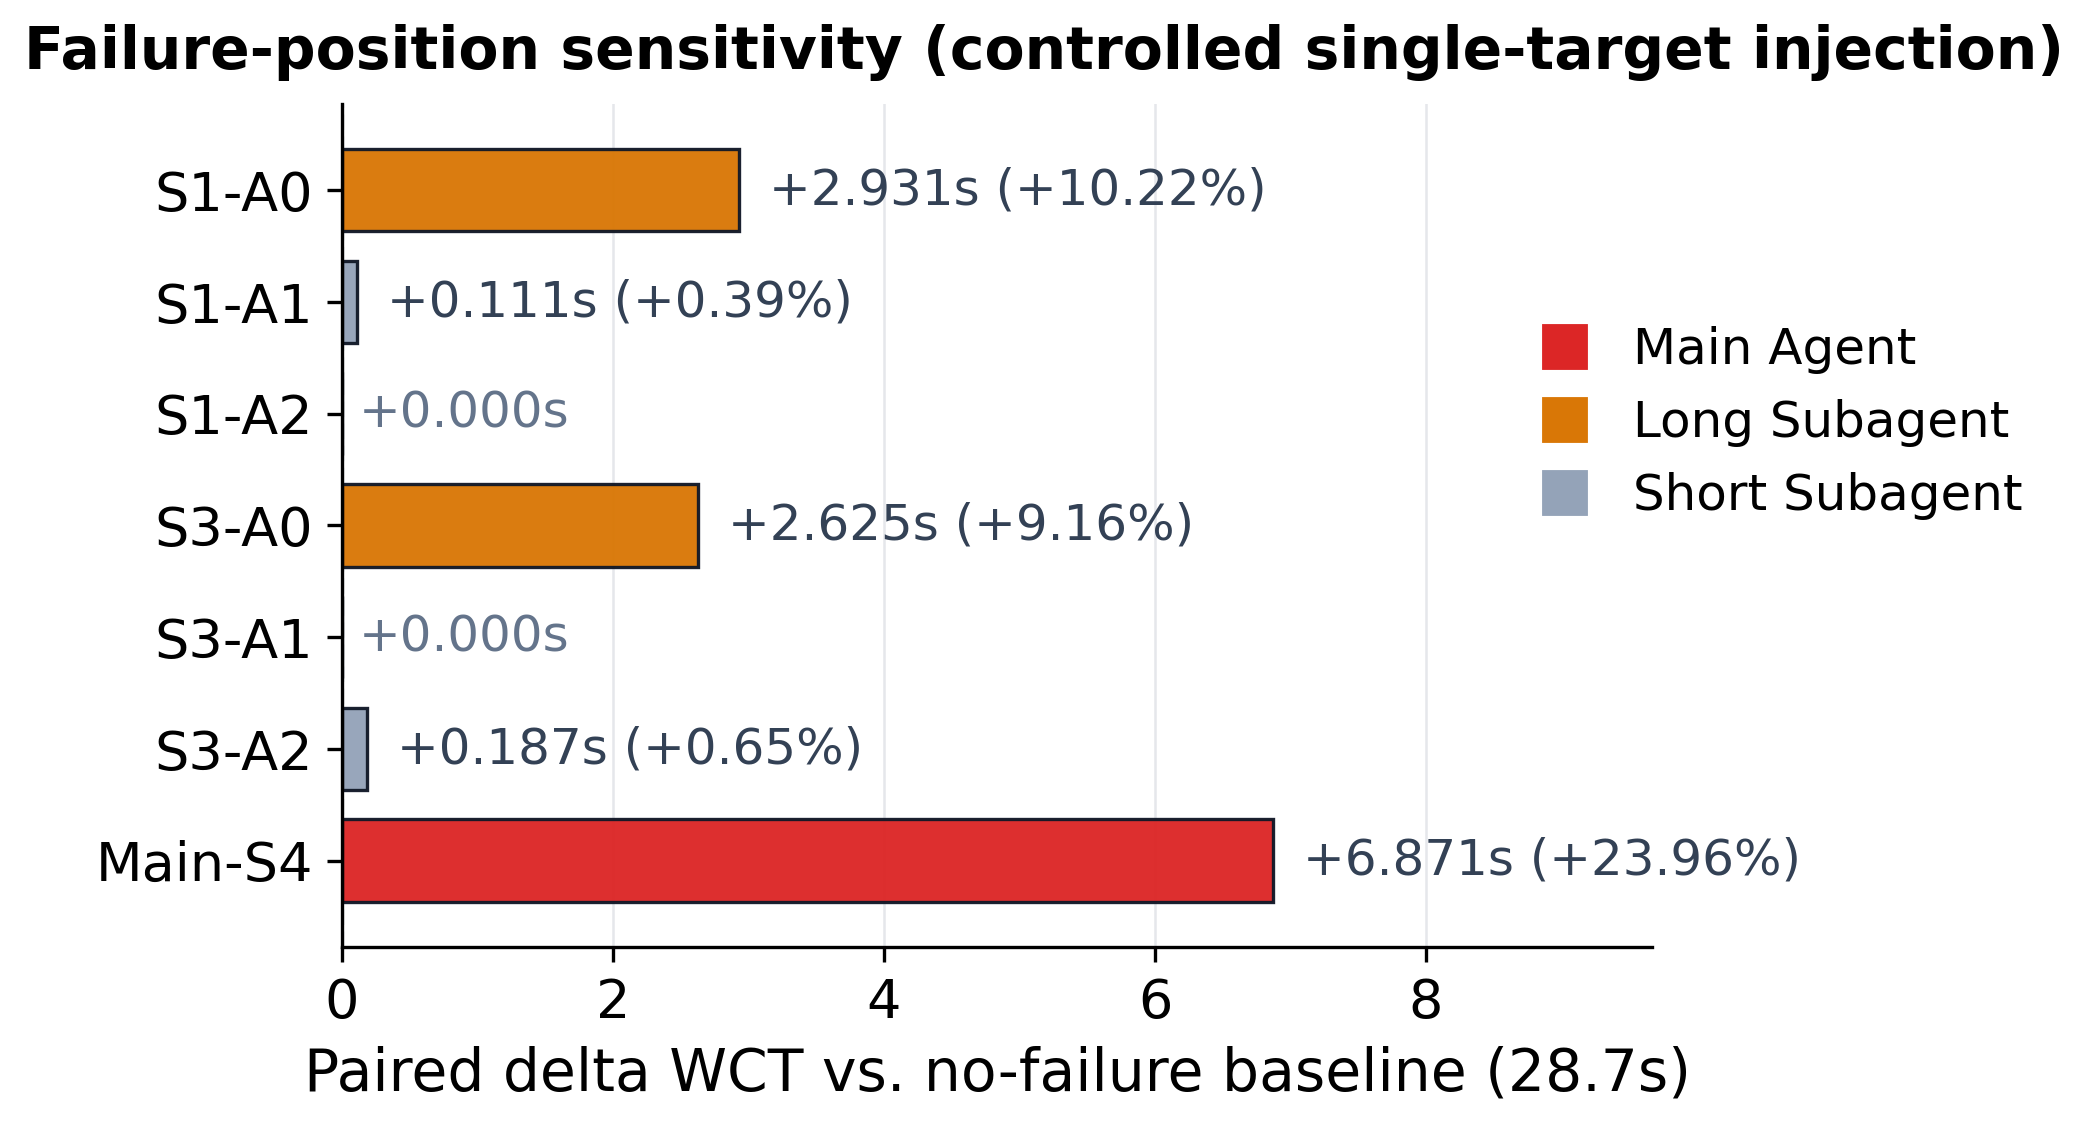
\includegraphics[width=\textwidth]{Figures/fig_motivation_agent_failure_impact.png}
      \end{figure}
    \end{column}
    \begin{column}{0.48\textwidth}
      \vspace{0.2cm}
      \scriptsize
      DP=8 online SGLSim 运行 1-3-1-3-1 workflow：每个 subagent 约 40K tokens，最终 main-agent 聚合上下文接近 120K tokens。曲线把 final main-agent failure、long-tail critical subagent failure 和普通 fan-out subagent 区分开，说明相同 workflow 结构中的故障点会产生不同 WCT 惩罚。
    \end{column}
  \end{columns}
\end{frame}

%------------------------------------------------------------
\section{Problem Formulation}
%------------------------------------------------------------

\begin{frame}{Objective：Workflow Completion Time}
  \small
  AegisKV 优化所有 workflow 的平均 completion time，而不是单个 request 的 recovery latency：

  \vspace{0.12cm}
  \[
    \min \ \operatorname{Avg}(\operatorname{WCT})
    \;=\;
    \min \ \frac{1}{|\mathcal{W}|}\sum_{i=1}^{|\mathcal{W}|} \operatorname{WCT}_i .
  \]

  \vspace{0.10cm}
  \begin{itemize}
    \item 不同任务的 workflow 规模与结构差异很大，用平均 WCT 比 P99 更能反映整体 serving 质量。
    \item 单个 workflow 的 WCT 仍由 \textbf{critical path} 决定，而非 request-level latency 之和。
    \item GPUReplica 只保护 Critical Agent 的高价值 KV segment；HostBackup 固定 write-through；$\alpha$ 控制 GPU backup HBM 预算。
  \end{itemize}
\end{frame}

\begin{frame}{AegisKV 三层在线决策}
  \small
  给定 workflow metadata，AegisKV 依次执行三个算法：

  \vspace{0.10cm}
  \begin{enumerate}
    \item \textbf{Criticality}：识别 Critical Agent（当前实验：静态 workflow 预标注）
    \item \textbf{Segment Backup}：frontier 扩展时在线 admit/evict GPUReplica（$U(\Delta n)/|\Delta n|$）
    \item \textbf{$\alpha$ 控制}：根据 critical pressure 与 failure exposure 划分 Backup HBM
  \end{enumerate}

  \vspace{0.12cm}
  \begin{columns}[T,onlytextwidth]
    \begin{column}{0.32\textwidth}
      \smallcard{Algo 1}{Critical Agent\\}
    \end{column}
    \begin{column}{0.32\textwidth}
      \smallcard{Algo 2}{Segment set $\mathcal{C}_t$\\GPUReplica}
    \end{column}
    \begin{column}{0.32\textwidth}
      \smallcard{Algo 3}{$(h_t, P_{\mathrm{fail}})$\\$\rightarrow \alpha_t$}
    \end{column}
  \end{columns}

  \vspace{0.08cm}
  \footnotesize
  Algo 1 Select Critical Agent $\rightarrow$ Algo 2 Select KV segment $\rightarrow$ Algo 3 Decide Backup HBM budget $\alpha_t$。
\end{frame}

\begin{frame}{算法 1：Workflow Critical Path 与 WCT}
  \small
  单个 workflow 的 completion time 由 \textbf{critical path} 决定：

  \vspace{0.06cm}
  \[
    \operatorname{WCT} = \sum_{a' \in \pi_{\mathrm{crit}}} T(a')
    + \mathbf{1}[\mathrm{fail}(a)] \cdot T_{\mathrm{retry}}(a).
  \]

  \vspace{0.04cm}
  \footnotesize
  $\pi_{\mathrm{crit}}$：critical path agent 序列；
  $T(a')$：agent 执行时间；
  $T_{\mathrm{retry}}(a)$：failure 后 retry 开销。（当前基于静态 workflow，后续增加Criticality Predictor）

  \vspace{0.08cm}
  \begin{figure}
    \centering
    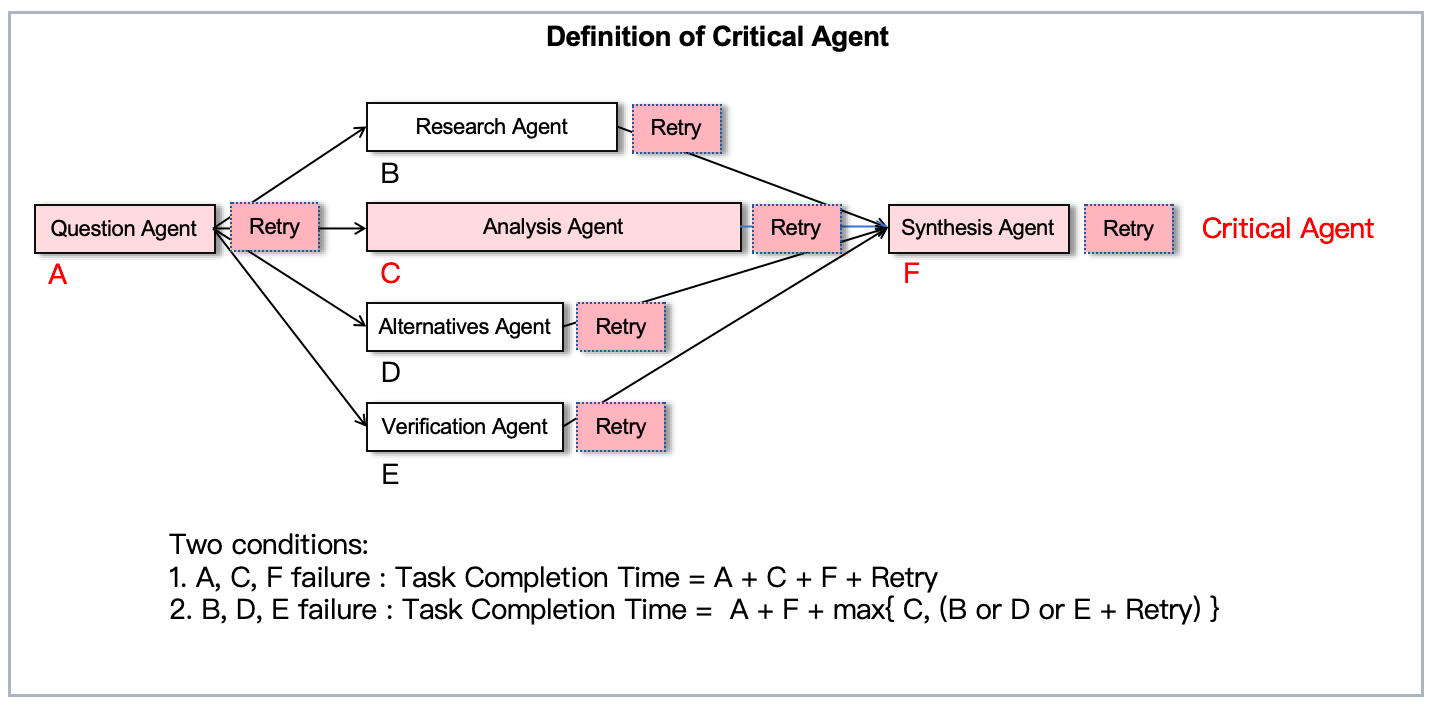
\includegraphics[width=0.88\textwidth]{Figures/critical_agent_definition.png}
  \end{figure}

\end{frame}

\begin{frame}{算法 2（1/5）：在线 Segment Placement 问题}
  \small
  \textbf{不是 offline knapsack}：KV 随 prefill/decode 不断 extend radix frontier，候选集\textbf{随时间增长}。

  \vspace{0.08cm}
  \textbf{Decision epoch} $t$ 在 frontier 扩展事件触发（新 token 写入、D2H ACK 等）：
  \[
    \mathcal{N}_{t-1} \subseteq \mathcal{N}_t,
    \qquad
    \Delta\mathcal{N}_t = \mathcal{N}_t \setminus \mathcal{N}_{t-1}.
  \]

  \vspace{0.06cm}
  每个 segment / chunk $n \in \mathcal{N}_t$：
  \[
    n = (\operatorname{workflow},\,\operatorname{agent},\,\operatorname{span},\,\operatorname{owner},\,\operatorname{size}_t)
  \]
  其中 $\operatorname{size}_t$ 随 decode 推进而\textbf{单调增加}。

  \vspace{0.06cm}
  \textbf{候选过滤}（Algo 1）：
  $\mathcal{C}_t = \{ n \in \mathcal{N}_t \mid \operatorname{critical}(n)=1 \}$，
  Non-Critical 恒有 $x_{n,t}=0$。

  \vspace{0.04cm}
  \footnotesize
  每 epoch 对\textbf{新增 frontier chunk} $\Delta n$ 做 admission；HostBackup 随 write-through 同步延伸。
\end{frame}

\begin{frame}{算法 2（2/5）：Budget 约束与持有状态}
  \small
  Backup partition 在任意 epoch $t$ 满足\textbf{持有约束}（非一次性分配）：
  \[
    \sum_{n \in \mathcal{P}_t} \operatorname{size}^{\mathrm{gpu}}_t(n)
    \le
    M_{\mathrm{Backup}}(t) = \alpha_t M .
  \]

  \vspace{0.06cm}
  $\mathcal{P}_t$：epoch $t$ 已被 GPUReplica ACK 保护的 segment/chunk 集合；
  $\operatorname{size}^{\mathrm{gpu}}_t(n)$：$n$ 在 GPU 侧实际占用的 unique token 数。

  \vspace{0.08cm}
  \textbf{在线演化}：
  \begin{itemize}
    \item \textbf{Admit}：新 frontier $\Delta n$ 到达，$U(\Delta n,t)>0$ 且 budget 有余量
    \item \textbf{Extend}：同一 agent decode 推进，protected hot tail 随 frontier 延伸
    \item \textbf{Evict}：budget 不足时，淘汰当前 $\mathcal{P}_t$ 中 $\rho$ 最低的条目
    \item \textbf{Invalidate}：Host evict / failure 导致 safe frontier 失效时移出 $\mathcal{P}_t$
  \end{itemize}

  \vspace{0.04cm}
  \footnotesize
  HostBackup 不占 $M_{\mathrm{Backup}}$；GPUReplica 才计入上述持有约束。
\end{frame}

\begin{frame}{算法 2（3/5）：Recovery 价值}
  \small
  GPUReplica 保护的\textbf{收益}：failure 时相对 HostBackup restore 能节省多少时延。

  \vspace{0.08cm}
  \[
    V_g(\Delta n,t)
    =
    w(n)
    \cdot
    \bigl(
      C_{\mathrm{restore}}^{\mathrm{host}}(|\Delta n|, t)
      -
      C_{\mathrm{restore}}^{\mathrm{gpu}}(g, |\Delta n|, t)
    \bigr)
  \]

  \vspace{0.06cm}
  \scriptsize
  \renewcommand{\arraystretch}{1.12}
  \begin{tabular}{p{0.30\textwidth}p{0.62\textwidth}}
    \toprule
    项 & 含义 \\
    \midrule
    $w(n)$ & Algo 1 Critical 权重（main / long-decode / fan-out） \\
    $C_{\mathrm{restore}}^{\mathrm{host}}$ & failure 后从 HostBackup restore（H2D）的时延 \\
    $C_{\mathrm{restore}}^{\mathrm{gpu}}(g)$ & failure 后从 peer $g$ 的 GPUReplica restore（P2P）时延 \\
    \bottomrule
  \end{tabular}

  \vspace{0.08cm}
  \footnotesize
  不同 peer $g$ 的 KV locality、load、backup 覆盖不同 $\Rightarrow$ $C_{\mathrm{restore}}^{\mathrm{gpu}}(g)$ 不同 $\Rightarrow$ $V_g$ 不同。
\end{frame}

\begin{frame}{算法 2（4/5）：Backup 成本}
  \small
  GPUReplica 保护的\textbf{代价}：主动 copy 与 backup HBM 占用。

  \vspace{0.08cm}
  \[
    C_{\mathrm{backup}}^g(\Delta n,t)
    =
    C_{\mathrm{copy}}^g(\Delta n,t)
    +
    C_{\mathrm{hbm}}^g(\Delta n,t)
  \]

  \vspace{0.06cm}
  \scriptsize
  \renewcommand{\arraystretch}{1.12}
  \begin{tabular}{p{0.28\textwidth}p{0.64\textwidth}}
    \toprule
    项 & 含义 \\
    \midrule
    $C_{\mathrm{copy}}^g$ & 复制到 peer $g$ 的 P2P 带宽 / 时延（随 locality 变化） \\
    $C_{\mathrm{hbm}}^g$ & peer $g$ 的 Backup partition（$\alpha_t M_g$）占用成本 \\
    \bottomrule
  \end{tabular}

  \vspace{0.10cm}
  对每个候选 peer $g$，计算：
  \[
    U_g(\Delta n,t) = V_g(\Delta n,t) - C_{\mathrm{backup}}^g(\Delta n,t),
    \qquad
    \rho_g(\Delta n,t) = \frac{U_g(\Delta n,t)}{|\Delta n|}.
  \]

  \vspace{0.04cm}
  \footnotesize
  HostBackup 为固定 write-through 底座，不计入 $C_{\mathrm{backup}}^g$。
\end{frame}

\begin{frame}{算法 2（5/5）：Peer 选择与 Event-Driven Admission}
  \small
  \textbf{Peer 选择}：在 healthy peer 集合 $\mathcal{G}_t$ 上取 value-density 最大者：
  \[
    g_t^* = \arg\max_{g \in \mathcal{G}_t} \rho_g(\Delta n,t),
    \qquad
    U^* = U_{g_t^*}(\Delta n,t).
  \]

  \vspace{0.08cm}
  \textbf{Online admission}（每个 frontier 扩展事件）：
  \begin{enumerate}
    \item 对每个 $g \in \mathcal{G}_t$ 计算 $\rho_g(\Delta n,t)$
    \item 选 $g_t^* = \arg\max_g \rho_g$；若 $U^*>0$ 且 $g_t^*$ 有 budget $\rightarrow$ \textbf{admit}
    \item 否则若 $\rho_{g_t^*}$ 高于 $\mathcal{P}_t$ 中最低 $\rho$ $\rightarrow$ \textbf{replace/evict}
    \item ACK 后在 $g_t^*$ 上更新 safe frontier；failure 时取 $\arg\min C_a$
  \end{enumerate}

  \vspace{0.06cm}
  \footnotesize
  不同 peer 通过 $C_{\mathrm{restore}}^{\mathrm{gpu}}(g)$ 与 $C_{\mathrm{backup}}^g$ 影响 $\rho_g$；最终 backup 落在 $\rho_g$ 最高的 peer 上。
\end{frame}

\begin{frame}{算法 3：MDP 决定 Backup HBM 比例 $\alpha_t$}
  \small
  对 GPU $g$，AegisKV 把可控 HBM budget $M_g$ 划分为：

  \vspace{0.10cm}
  \[
    M_{\mathrm{Backup}}(g,t) = \alpha_{g,t} M_g,
    \qquad
    M_{\mathrm{Inference}}(g,t) = (1-\alpha_{g,t})M_g .
  \]

  \vspace{0.10cm}
  \begin{block}{Key Trade-off}
    1. Workload ↑ or Failure ↓ -> $\alpha$ ↓ \\
    2. Workload ↓ or Failure ↑ -> $\alpha$ ↑
  \end{block}

  \vspace{0.10cm}
  \footnotesize
  全局 action 是 $\boldsymbol{\alpha}_t=(\alpha_{1,t},\ldots,\alpha_{G,t})$
\end{frame}

\begin{frame}{算法 3：MDP 决定 Backup HBM 比例 $\alpha_t$}
  \small
  在线控制器可以写成 MDP(Markov Decision Process)\cite{yu2026poolcachesadaptivehbm}：

  \vspace{0.04cm}
  \[
    (\mathcal{S},\mathcal{A},\mathcal{P},\mathcal{R},\gamma),
    \qquad
    J(\pi)=\mathbb{E}_{\pi}\left[\sum_{t=0}^{\infty}\gamma^t r_t\right].
  \]

  \vspace{-0.05cm}
  \scriptsize
  \renewcommand{\arraystretch}{1.10}
  \begin{tabular}{p{0.15\textwidth}p{0.72\textwidth}}
    \toprule
    状态 $\mathcal{S}$ 分量 & AegisKV 中的含义 \\
    \midrule
    $h_t$ & Request pressure \\
    $k_t$ & Inference partition 中的 KV / prefix hit rate \\
    $e_t$ & candidate retry tokens 上的 effective backup coverage \\
    $L_t$ & Context length 或 token-length pressure \\
    $\alpha_t$ & backup/inference allocation ratio \\
    \bottomrule
  \end{tabular}

\end{frame}


% \begin{frame}{三个算法的执行顺序}
%   \small
%   \begin{center}
%   \begin{tikzpicture}[
%     node distance=0.55cm and 0.35cm,
%     box/.style={draw=hkblue, fill=softblue, rounded corners, align=center,
%                 font=\scriptsize, inner sep=4pt, minimum width=2.1cm},
%     arr/.style={-{Stealth[length=2mm]}, thick, draw=hkblue}
%   ]
%     \node[box] (wf) {Workflow\\metadata};
%     \node[box, right=of wf] (a1) {Algo 1\\Static label};
%     \node[box, right=of a1] (a2) {Algo 2\\Segment pick\\$\mathcal{C}_t$};
%     \node[box, right=of a2] (a3) {Algo 3\\$\alpha_t$};
%     \node[box, below=0.7cm of a2] (exec) {GPUReplica + HostBackup\\failure-time restore};
%     \draw[arr] (wf) -- (a1);
%     \draw[arr] (a1) -- (a2);
%     \draw[arr] (a2) -- (a3);
%     \draw[arr] (a3) -- (exec);
%     \draw[arr] (a1.south) |- (exec.west);
%   \end{tikzpicture}
%   \end{center}

%   \vspace{0.12cm}
%   \begin{itemize}
%     \item Algo 1：静态 workflow 预标注 Critical Agent；后续 predictor 替代静态标签。
%     \item Algo 2：仅在 $\mathcal{C}_t$ 内按 $\rho(n)$ 贪心选 GPUReplica segment。
%     \item Algo 3：静态标签映射 $h_t$，结合 $P_{\mathrm{fail}}$ 查表得 $\alpha_t$。
%   \end{itemize}
% \end{frame}

% %------------------------------------------------------------
% \section{System Overview}
% %------------------------------------------------------------

% \begin{frame}{System Overview}
%   \small
%   \begin{figure}
%     \centering
%     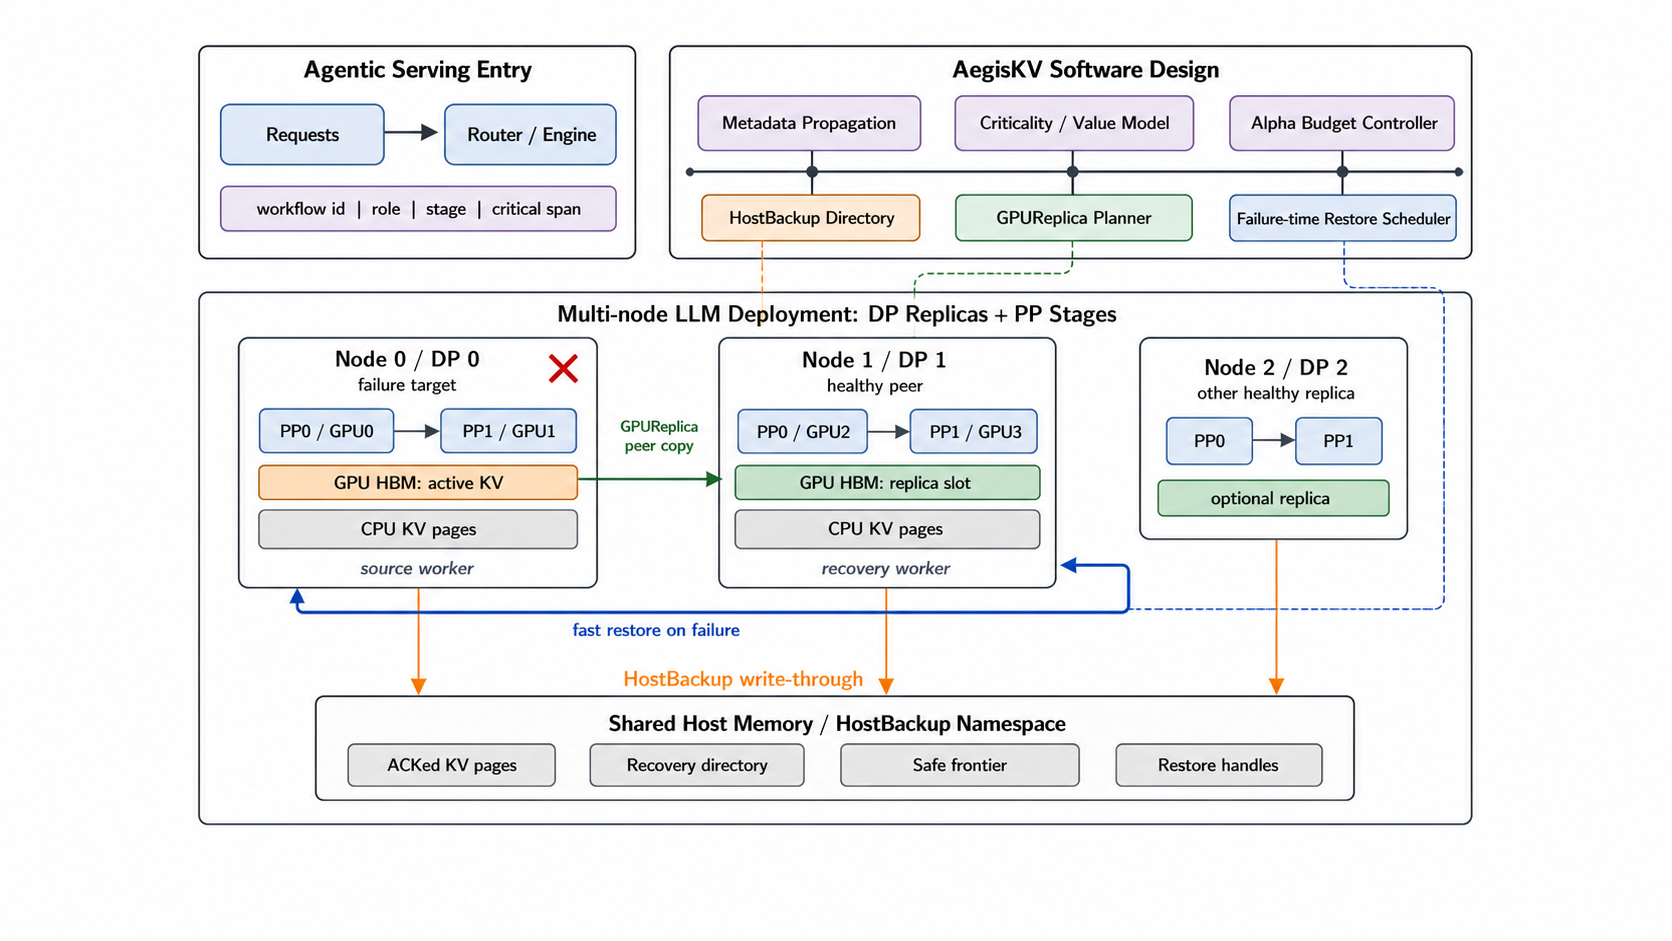
\includegraphics[width=0.9\textwidth]{Figures/fig_system_overview_imagegen_margin_prompt.png}
%   \end{figure}

%   \vspace{0.06cm}
%   \footnotesize
%   AegisKV 在 GPUReplica、HostBackup 提供 workflow-aware fault tolerance。

% \end{frame}

%------------------------------------------------------------
\section{Implementation}
%------------------------------------------------------------

\begin{frame}{AegisKV 基于 SGLang 实现}
  \scriptsize
  SGLang ->AegisKV 
  \vspace{0.4cm}

  \vspace{0.06cm}
  \renewcommand{\arraystretch}{1.08}
  \begin{tabular}{
    >{\raggedright\arraybackslash}p{0.22\textwidth}
    >{\raggedright\arraybackslash}p{0.24\textwidth}
    >{\raggedright\arraybackslash}p{0.42\textwidth}
  }
    \toprule
    SGLang & AegisKV & 实现行为 \\
    \midrule
    Radix prefix cache & Workflow metadata propagation & 写入 workflow id、stage、role、turn、critical span 等 \\
    HiCache write-through D2H & HostBackup directory & ACK 后把 source-rank Host KV 发布为 cross-rank recoverable frontier \\
    HiCache load / H2D restore & Failure-time restore scheduler & 将 failed-rank Host KV 恢复到 retry rank \\
    DP controller / scheduler & Retry routing & 路由 retry \\
    GPU KV pool / HBM budget & GPUReplica + $\alpha$ partition & 在 $(1-\alpha)M_g$ inference 与 $\alpha M_g$ backup 间划分 HBM；复制 selected Critical KV 到 peer GPU \\
    \bottomrule
  \end{tabular}

  \vspace{0.4cm}
  \footnotesize
  GPUReplica + HostBackup
\end{frame}

%------------------------------------------------------------
\section{Evaluation}
%------------------------------------------------------------

\begin{frame}{Evaluation: Vary Allocation Ratio $\alpha$}

  \begin{figure}
    \centering
    \begin{columns}[T,onlytextwidth]
      \begin{column}{0.49\textwidth}
        \centering
        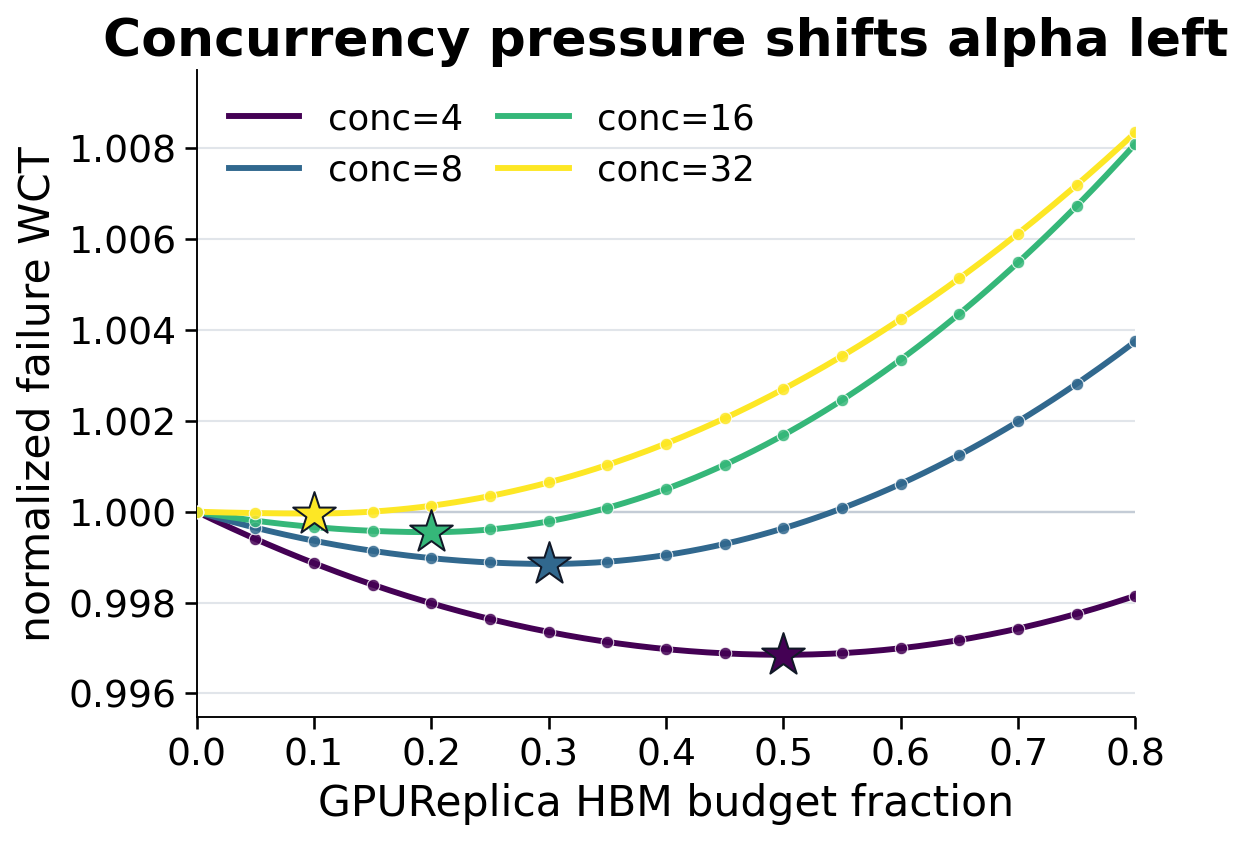
\includegraphics[width=\linewidth]{Figures/fig_gpu_replica_alpha_tradeoff_concurrency.png}

        \vspace{0.2em}
      \end{column}
      \begin{column}{0.49\textwidth}
        \centering
        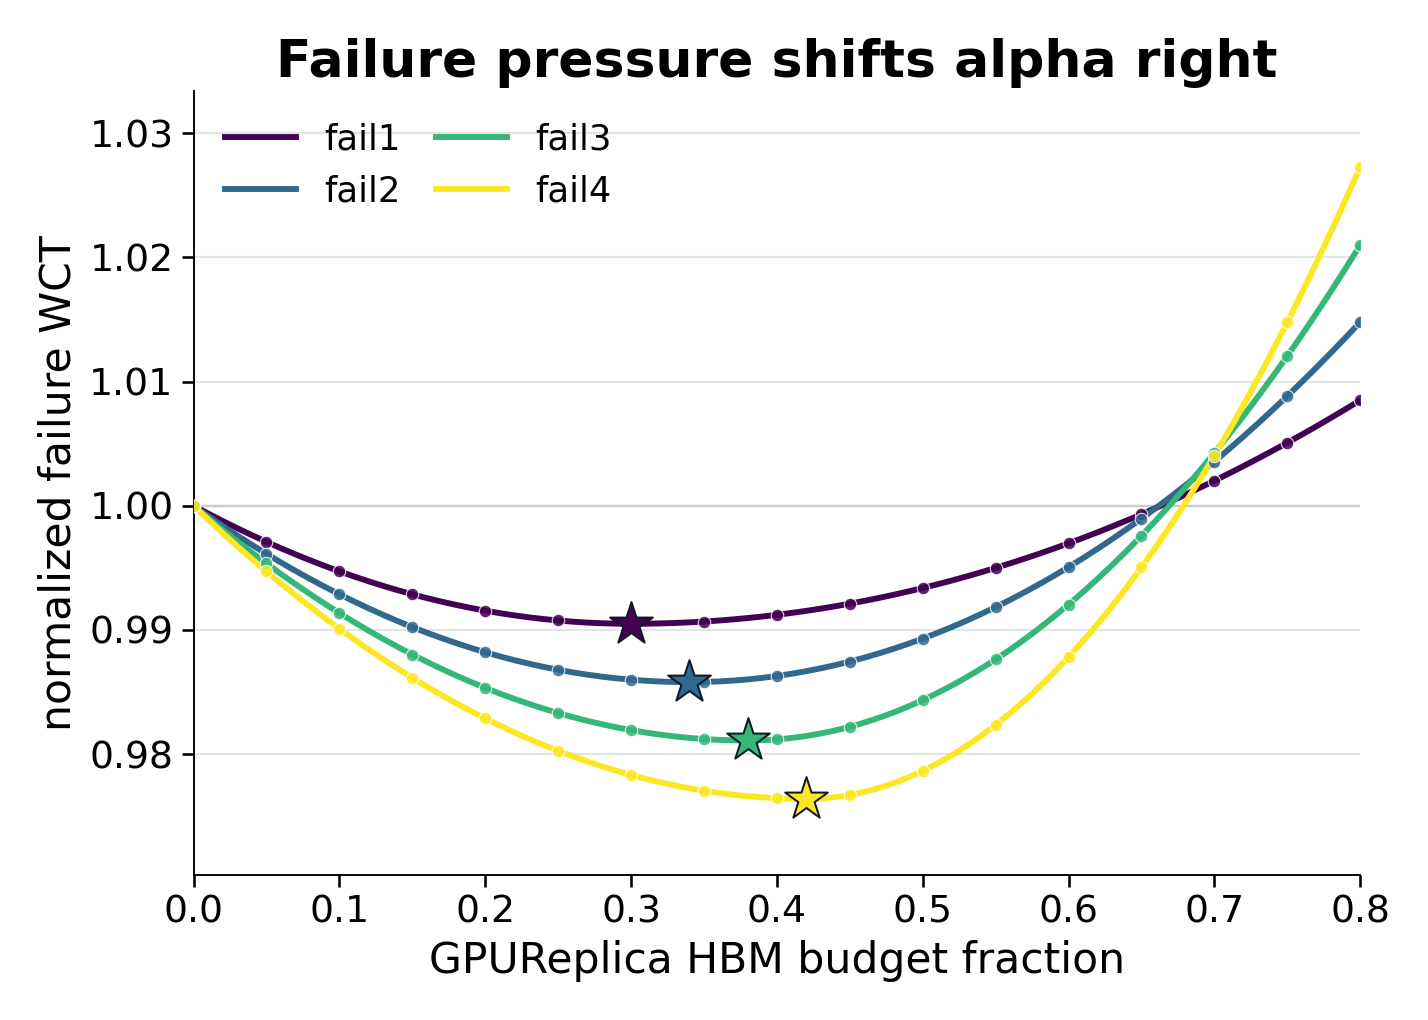
\includegraphics[width=\linewidth]{Figures/fig_gpu_replica_alpha_tradeoff_failure.png}

        \vspace{0.2em}
      \end{column}
    \end{columns}
  \end{figure}

  \vspace{0.06cm}
  \footnotesize
  \begin{block}{Trade-off}
    1. Workload ↑ or Failure ↓-> $\alpha$ ↓ \\
    2. Workload ↓ or Failure ↑ -> $\alpha$ ↑
  \end{block}
\end{frame}

\begin{frame}{Evaluation: Vary Backup Policy}
  \begin{figure}
    \centering
    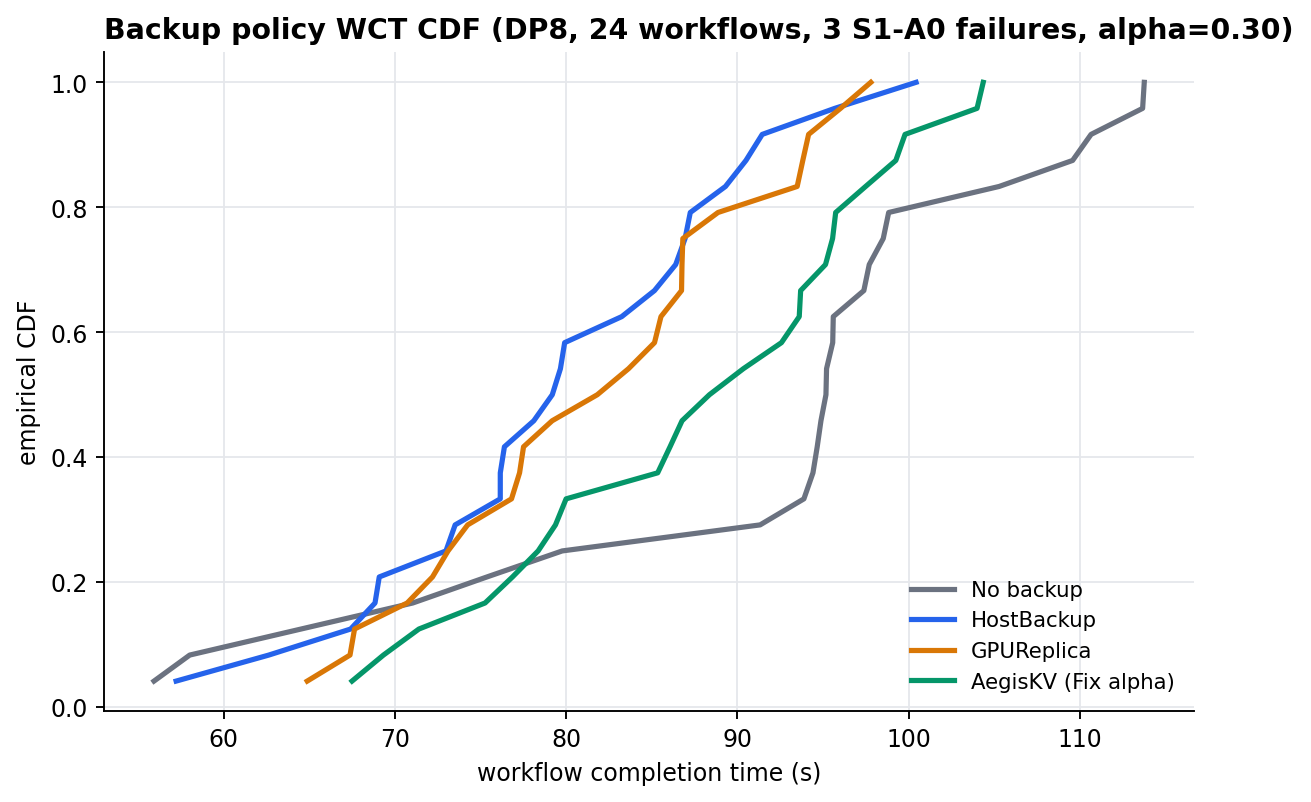
\includegraphics[width=\linewidth]{Figures/fig_backup_policy_comparison.png}
  \end{figure}
\end{frame}

\begin{frame}{Evaluation: Vary $\alpha$ in AegisKV}
  \begin{figure}
    \centering
    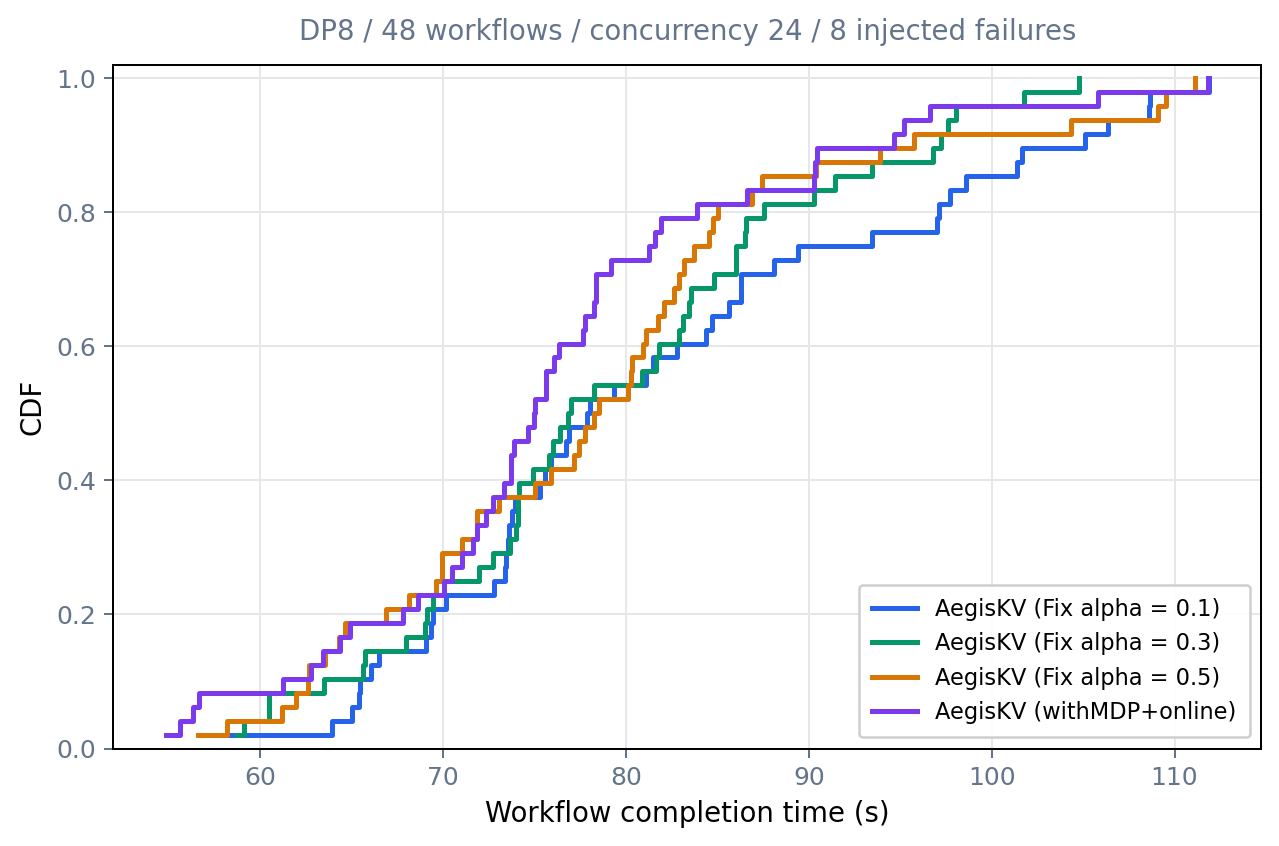
\includegraphics[width=\linewidth]{Figures/fig_aegiskv_alpha_policy_wct_cdf.png}
  \end{figure}
\end{frame}

\begin{frame}{Evaluation: Real CC Trace (Weka Subagent)}
  \begin{figure}
    \centering
    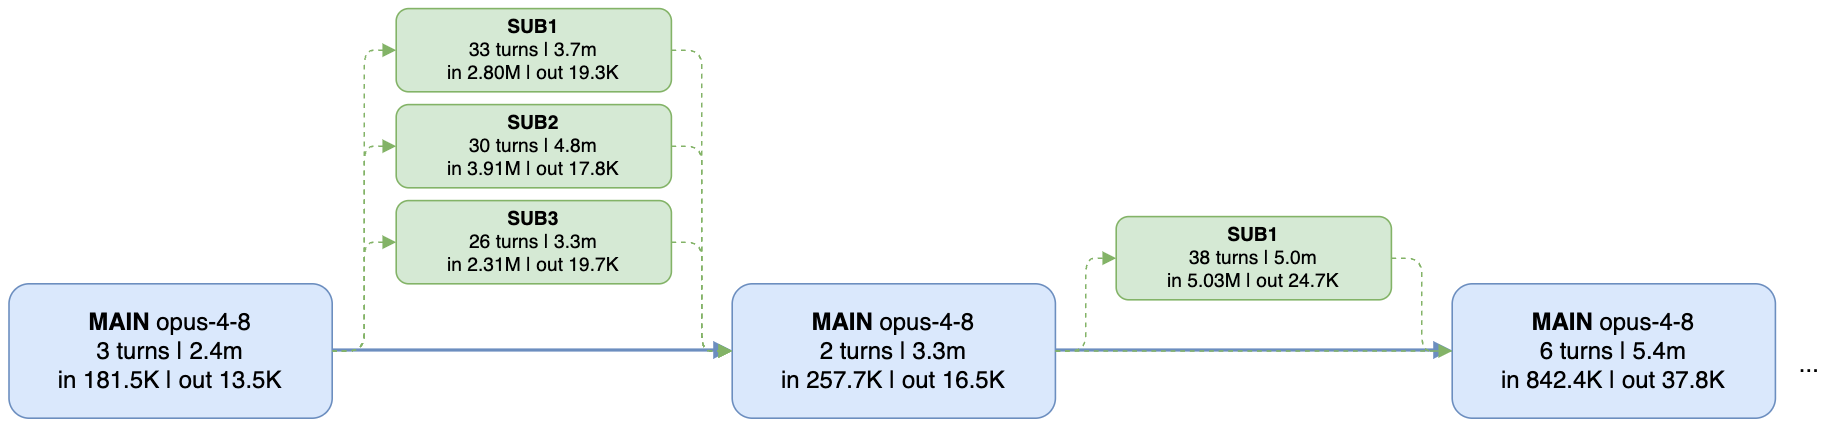
\includegraphics[width=\linewidth]{Figures/real_trace.png}
  \end{figure}

  \vspace{0.04cm}
  \footnotesize
\end{frame}

\begin{frame}{Evaluation: Real CC Trace (Weka Subagent)}
  \begin{figure}
    \centering
    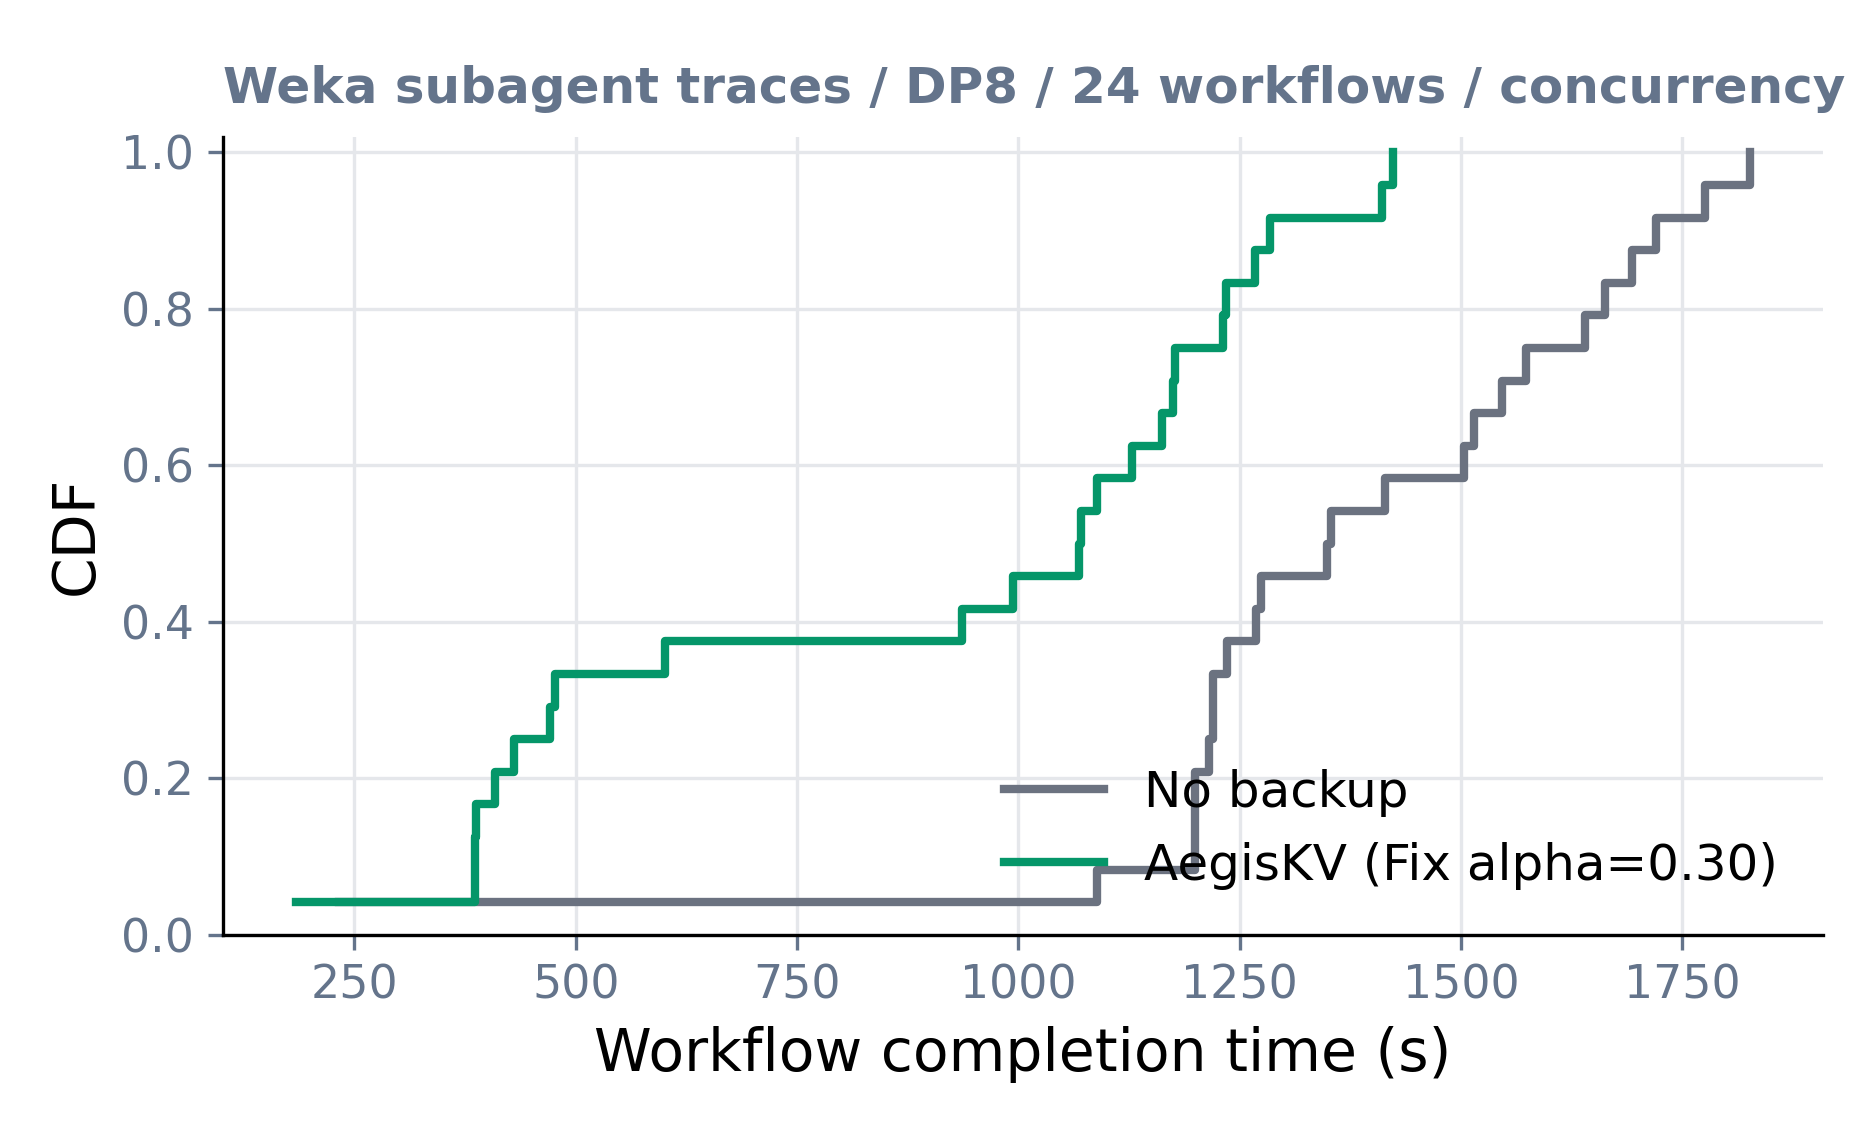
\includegraphics[width=\linewidth]{Figures/fig_weka_subagent_policy_wct_cdf.png}
  \end{figure}

  \vspace{0.04cm}
  \footnotesize
  cc-traces-weka-062126，24 workflows / DP8 / 6 soft failures；
  No backup vs AegisKV ($\alpha{=}0.30$)：Mean WCT 1372s $\rightarrow$ 891s，P90 1712s $\rightarrow$ 1279s。
\end{frame}

%------------------------------------------------------------
\section{Next Step}
%------------------------------------------------------------

\begin{frame}{Next Step}
  \begin{itemize}
    \item Algo 1: 根据Real trace 设计Criticality Predictor，在线预测 critical path。
    \item Algo 2: 分析每个影响因素，更 solid 的算法和实验。
    \item Algo 3: 尝试整合到 Algo 2 中。
  \end{itemize}
\end{frame}

\begin{frame}[allowframebreaks]{References}
  \nocite{*}
  \bibliographystyle{Simple}
  \bibliography{ref}
\end{frame}

\end{document}
